\documentclass[12pt]{article}
\usepackage[utf8]{inputenc}
\usepackage{amsmath, amssymb, amsfonts, amsthm}
\usepackage{graphicx}
\usepackage{geometry}
\geometry{a4paper, margin=2.5cm}
\usepackage{titlesec}
\titleformat{\section}{\large\bfseries}{\thesection}{1em}{}
\titleformat{\subsection}{\normalsize\bfseries}{\thesubsection}{1em}{}
\usepackage{braket}
\usepackage{pgfplots}
\pgfplotsset{compat=1.17}
\usepackage{tikz}
\usetikzlibrary{shapes,arrows,positioning,calc}

\newtheorem{definicao}{Definição}
\newtheorem{teorema}{Teorema}
\newtheorem{observacao}{Observação}

\begin{document}

\title{Aula 6 -- Aproximações de Campo Médio e Soluções Exatas em Modelos de Ising:
da desigualdade de Gibbs-Bogoliubov ao modelo de Curie-Weiss}
\author{Notas de Aula -- Tópicos em Mecânica Estatística \\ Aula ministrada por Silvio Salinas \\ Autor: Thiago Siqueira Domingues}
\date{}

\maketitle

\begin{abstract}
Nesta aula, exploramos o formalismo variacional baseado na desigualdade de Gibbs-Bogoliubov como ferramenta para construir aproximações de campo médio. Aplicamos o método ao modelo de Blume-Capel (spin-1 com campo cristalino), obtendo a energia livre variacional e a equação de estado. Em seguida, generalizamos para o modelo de Curie-Weiss com interações de longo alcance, onde a solução é exata via método de Laplace. Analisamos a expansão de Landau da energia livre e construímos o diagrama de fases, identificando linhas de transição de primeira e segunda ordem e um ponto tricrítico. Por fim, estendemos a discussão para sistemas com campo aleatório, onde a desordem é tratada via média sobre distribuições binárias.
\end{abstract}

\section{Introdução}

O modelo de Ising, em sua forma mais simples com interações de curto alcance, é exatamente solúvel apenas em 1D (sem transição de fase) e em 2D com campo nulo (solução de Onsager). Para situações mais complexas — campo finito, 3D ou sistemas com anisotropia — recorremos a aproximações. Uma das mais poderosas é a aproximação de campo médio, que pode ser justificada via princípio variacional de Gibbs-Bogoliubov.

Nesta aula, desenvolvemos o formalismo variacional e o aplicamos a dois sistemas:
\begin{enumerate}
    \item O modelo de Blume-Capel, um sistema de spin-1 com parâmetro de campo cristalino $D$.
    \item O modelo de Curie-Weiss, com interações de longo alcance, que é exatamente solúvel e reproduz os resultados de campo médio.
\end{enumerate}

Ao final, discutimos a generalização para sistemas com campo aleatório.

\section{Desigualdade de Gibbs-Bogoliubov}

\begin{teorema}[Desigualdade de Gibbs-Bogoliubov]
Seja $\mathcal{H}$ um Hamiltoniano arbitrário e $\mathcal{H}_0$ um Hamiltoniano de teste. Então, a energia livre de Helmholtz associada a $\mathcal{H}$ satisfaz
\begin{equation}
    F(\mathcal{H}) \leq F(\mathcal{H}_0) + \langle \mathcal{H} - \mathcal{H}_0 \rangle_0,
\end{equation}
onde $\langle \cdot \rangle_0$ denota a média térmica calculada com o Hamiltoniano $\mathcal{H}_0$.
\end{teorema}

\begin{proof}
A demonstração segue da convexidade da função logaritmo e da positividade da entropia relativa de Kullback-Leibler. Considere as distribuições
\begin{equation}
    P(\{\sigma\}) = \frac{e^{-\beta \mathcal{H}}}{Z}, \quad P_0(\{\sigma\}) = \frac{e^{-\beta \mathcal{H}_0}}{Z_0}.
\end{equation}
Temos
\begin{equation}
    \frac{1}{N} \sum_{\{\sigma\}} P(\{\sigma\}) \ln \frac{P(\{\sigma\})}{P_0(\{\sigma\})} \geq 0,
\end{equation}
o que implica
\begin{equation}
    -\frac{1}{\beta} \ln Z \leq -\frac{1}{\beta} \ln Z_0 + \langle \mathcal{H} - \mathcal{H}_0 \rangle_0.
\end{equation}
\end{proof}

Esta desigualdade é a base do método variacional: minimizamos o lado direito sobre os parâmetros livres em $\mathcal{H}_0$ para obter a melhor aproximação para a energia livre verdadeira.

\section{Modelo de Blume-Capel}

O modelo de Blume-Capel descreve um sistema de spins $S_i \in \{-1, 0, +1\}$ com Hamiltoniano
\begin{equation}
    \mathcal{H}_{\text{BC}} = -J \sum_{\langle i,j \rangle} S_i S_j + D \sum_{i=1}^N S_i^2,
\end{equation}
onde $D$ é o parâmetro de campo cristalino que penaliza estados com $S_i = \pm 1$ em relação a $S_i = 0$.

\subsection{Hamiltoniano de Teste}

Escolhemos um Hamiltoniano de teste na forma de campo médio:
\begin{equation}
    \mathcal{H}_0 = -\eta \sum_{i=1}^N S_i + D \sum_{i=1}^N S_i^2,
\end{equation}
onde $\eta$ é um campo efetivo variacional. A função de partição associada é
\begin{equation}
    Z_0 = \sum_{\{S_i\}} e^{-\beta \mathcal{H}_0} = \left[ 1 + 2 e^{-\beta D} \cosh(\beta \eta) \right]^N.
\end{equation}
Portanto, a energia livre por sítio é
\begin{equation}
    f_0 = -\frac{1}{\beta} \ln Z_0 = -\frac{1}{\beta} \ln\left[ 1 + 2 e^{-\beta D} \cosh(\beta \eta) \right].
\end{equation}

\subsection{Médias com o Hamiltoniano de Teste}

Precisamos calcular as médias:
\begin{equation}
    \langle S_i \rangle_0 = \frac{2 e^{-\beta D} \sinh(\beta \eta)}{1 + 2 e^{-\beta D} \cosh(\beta \eta)} \equiv m,
\end{equation}
e
\begin{equation}
    \langle S_i^2 \rangle_0 = \frac{2 e^{-\beta D} \cosh(\beta \eta)}{1 + 2 e^{-\beta D} \cosh(\beta \eta)} \equiv q.
\end{equation}

\subsection{Energia Livre Variacional}

A energia livre de Gibbs variacional é
\begin{align}
    \phi(\eta) &= f_0 + \langle \mathcal{H}_{\text{BC}} - \mathcal{H}_0 \rangle_0 \\
    &= -\frac{1}{\beta} \ln\left[ 1 + 2 e^{-\beta D} \cosh(\beta \eta) \right] 
    - \frac{J q}{2} N \langle S_i \rangle_0^2 + \eta N \langle S_i \rangle_0.
\end{align}
Aproveitando a extensividade, a energia livre por sítio é
\begin{equation}
    \phi(\eta) = -\frac{1}{\beta} \ln\left[ 1 + 2 e^{-\beta D} \cosh(\beta \eta) \right]
    - \frac{J q}{2} m^2 + \eta m,
\end{equation}
onde $q = z$ é o número de coordenação da rede (no caso de interações de curto alcance).

A condição de mínimo $\partial \phi / \partial \eta = 0$ fornece a equação de estado
\begin{equation}
    m = \frac{2 e^{-\beta D} \sinh(\beta \eta)}{1 + 2 e^{-\beta D} \cosh(\beta \eta)}, \quad \eta = J q m.
\end{equation}
Portanto,
\begin{equation}
    m = \frac{2 e^{-\beta D} \sinh(\beta J q m)}{1 + 2 e^{-\beta D} \cosh(\beta J q m)}.
\end{equation}

\subsection{Expansão de Landau}

Expandimos $\phi(\eta)$ em potências de $m$. Para $h=0$, a energia livre tem a forma
\begin{equation}
    \phi(m) = \phi_0 + \frac{a}{2} m^2 + \frac{b}{4} m^4 + \frac{c}{6} m^6 + \cdots,
\end{equation}
com
\begin{align}
    a &= \frac{k_B T}{J q} - 2 e^{-\beta D}, \\
    b &= \frac{1}{3} \left[ 2 e^{-\beta D} - 4 e^{-2\beta D} \right] + \frac{1}{J q} \frac{1}{\beta} \frac{1}{1 + 2 e^{-\beta D}} \cdots,
\end{align}
e assim por diante.

\subsection{Diagrama de Fases}

O diagrama de fases no plano $(T, D)$ apresenta:
\begin{itemize}
    \item Uma linha de transição de segunda ordem onde $a = 0$ e $b > 0$.
    \item Uma linha de transição de primeira ordem onde $a > 0$, $b < 0$ e $c > 0$.
    \item Um ponto tricrítico onde $a = b = 0$ e $c > 0$.
\end{itemize}

\begin{figure}[h]
\centering
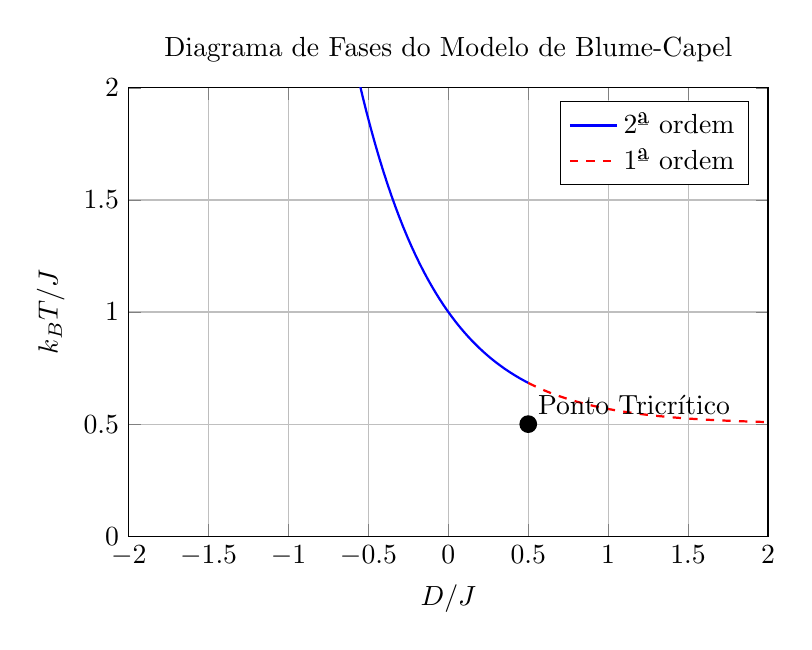
\begin{tikzpicture}
\begin{axis}[
    width=0.8\textwidth,
    height=0.6\textwidth,
    xlabel={$D/J$},
    ylabel={$k_B T / J$},
    xmin=-2, xmax=2,
    ymin=0, ymax=2,
    grid=both,
    legend pos=north east,
    title={Diagrama de Fases do Modelo de Blume-Capel}
]
\addplot[domain=-2:0.5, samples=100, color=blue, thick] {0.5*(1 + exp(-2*x))};
\addplot[domain=0.5:2, samples=100, color=red, thick, dashed] {0.5*(1 + exp(-2*x))};
\addplot[mark=*, mark size=3, only marks, color=black] coordinates {(0.5, 0.5)};
\node[above right] at (axis cs:0.5,0.5) {Ponto Tricrítico};
\addlegendentry{2ª ordem}
\addlegendentry{1ª ordem}
\end{axis}
\end{tikzpicture}
\caption{Diagrama de fases esquemático para o modelo de Blume-Capel. A linha azul contínua indica transições de segunda ordem, a linha vermelha tracejada indica transições de primeira ordem, e o ponto preto é o ponto tricrítico.}
\end{figure}

\section{Modelo de Curie-Weiss (Aproximação de Longo Alcance)}

O modelo de Curie-Weiss é definido pelo Hamiltoniano
\begin{equation}
    \mathcal{H}_{\text{CW}} = -\frac{J}{2N} \sum_{i=1}^N \sum_{j=1}^N S_i S_j + D \sum_{i=1}^N S_i^2.
\end{equation}
O termo de interação é de longo alcance e escalonado por $1/N$ para garantir extensividade.

\subsection{Função de Partição}

A função de partição é
\begin{equation}
    Z_N = \sum_{\{S_i\}} \exp\left[ \frac{\beta J}{2N} \left( \sum_i S_i \right)^2 - \beta D \sum_i S_i^2 \right].
\end{equation}
Usamos a identidade gaussiana:
\begin{equation}
    e^{\frac{\beta J}{2N} (\sum_i S_i)^2} = \sqrt{\frac{\beta J N}{2\pi}} \int_{-\infty}^{+\infty} dx \, e^{-\frac{\beta J N}{2} x^2 + \beta J x \sum_i S_i}.
\end{equation}
Assim,
\begin{equation}
    Z_N = \sqrt{\frac{\beta J N}{2\pi}} \int_{-\infty}^{+\infty} dx \, e^{-\frac{\beta J N}{2} x^2} \left[ 1 + 2 e^{-\beta D} \cosh\left( \beta J x \right) \right]^N.
\end{equation}

\subsection{Mudança de Variável}

Definimos $y = x$. A função de partição fica
\begin{equation}
    Z_N = \sqrt{\frac{\beta J N}{2\pi}} \int_{-\infty}^{+\infty} dy \, e^{-N \beta \phi(y)},
\end{equation}
com
\begin{equation}
    \phi(y) = \frac{J}{2} y^2 - \frac{1}{\beta} \ln\left[ 1 + 2 e^{-\beta D} \cosh(\beta J y) \right].
\end{equation}

\subsection{Método de Laplace}

No limite $N \to \infty$, a integral é dominada pelo mínimo de $\phi(y)$:
\begin{equation}
    g(T,D) = \lim_{N \to \infty} -\frac{1}{\beta N} \ln Z_N = \min_y \phi(y).
\end{equation}
A condição de mínimo $\partial \phi/\partial y = 0$ fornece
\begin{equation}
    y = \frac{2 e^{-\beta D} \sinh(\beta J y)}{1 + 2 e^{-\beta D} \cosh(\beta J y)}.
\end{equation}
Esta é a equação de estado do modelo de Curie-Weiss para spin-1.

\subsection{Expansão de Landau para o Modelo de Curie-Weiss}

A energia livre $\phi(y)$ pode ser expandida como
\begin{equation}
    \phi(y) = \phi_0 + \frac{1}{2} A y^2 + \frac{1}{4} B y^4 + \frac{1}{6} C y^6 + \cdots,
\end{equation}
onde
\begin{align}
    A &= J - \beta J^2 \frac{2 e^{-\beta D}}{1 + 2 e^{-\beta D}}, \\
    B &= -\frac{\beta^3 J^4}{3} \frac{2 e^{-\beta D}}{1 + 2 e^{-\beta D}} + \cdots, \\
    C &= \frac{\beta^5 J^6}{15} \frac{2 e^{-\beta D}(1 - 2 e^{-\beta D})}{(1 + 2 e^{-\beta D})^4} + \cdots.
\end{align}

\section{Generalização para Campo Aleatório}

Consideramos agora um campo externo que varia de sítio para sítio, $h_i$, com distribuição de probabilidade
\begin{equation}
    P(h_i) = \frac{1}{2} \delta(h_i - h) + \frac{1}{2} \delta(h_i + h).
\end{equation}
O Hamiltoniano é
\begin{equation}
    \mathcal{H} = -\frac{J}{2N} \left( \sum_i S_i \right)^2 - \sum_i h_i S_i.
\end{equation}

A função de partição para uma configuração fixa de campos é
\begin{equation}
    Z_N(\{h_i\}) = \sum_{\{S_i\}} \exp\left[ \frac{\beta J}{2N} \left( \sum_i S_i \right)^2 + \beta \sum_i h_i S_i \right].
\end{equation}
Usando novamente a identidade gaussiana e a mudança de variável $y$, obtemos
\begin{equation}
    Z_N(\{h_i\}) = \sqrt{\frac{\beta J N}{2\pi}} \int_{-\infty}^{+\infty} dy \, e^{-\frac{\beta J N}{2} y^2} \prod_{i=1}^N \left[ 2 \cosh\left( \beta J y + \beta h_i \right) \right].
\end{equation}
A média sobre a desordem ($\overline{Z_N}$) é
\begin{equation}
    \overline{Z_N} = \sqrt{\frac{\beta J N}{2\pi}} \int_{-\infty}^{+\infty} dy \, e^{-N \beta \phi_{\text{dis}}(y)},
\end{equation}
com
\begin{equation}
    \phi_{\text{dis}}(y) = \frac{J}{2} y^2 - \frac{1}{\beta} \left[ \frac{1}{2} \ln\left( 2 \cosh(\beta J y + \beta h) \right) + \frac{1}{2} \ln\left( 2 \cosh(\beta J y - \beta h) \right) \right].
\end{equation}

A equação de estado para a magnetização média é
\begin{equation}
    m = \frac{1}{2} \tanh( \beta J m + \beta h ) + \frac{1}{2} \tanh( \beta J m - \beta h ).
\end{equation}

\begin{figure}[h]
\centering
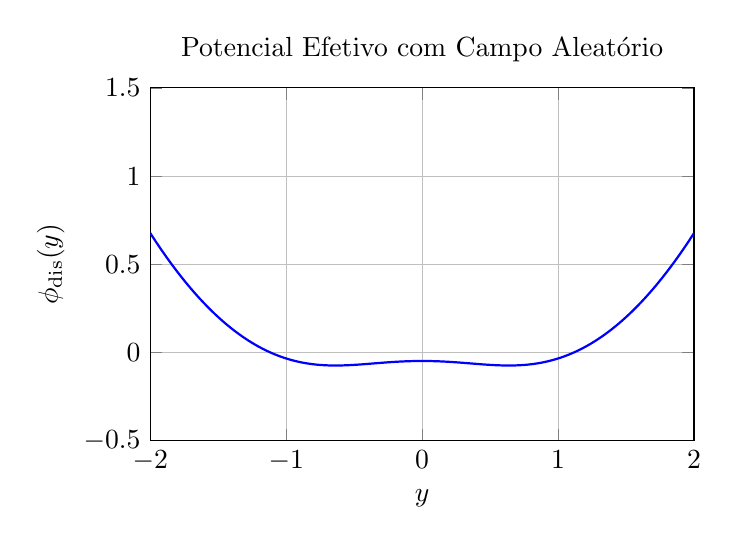
\begin{tikzpicture}
\begin{axis}[
    width=0.7\textwidth,
    height=0.5\textwidth,
    xlabel={$y$},
    ylabel={$\phi_{\text{dis}}(y)$},
    xmin=-2, xmax=2,
    ymin=-0.5, ymax=1.5,
    grid=both,
    title={Potencial Efetivo com Campo Aleatório}
]
\addplot[domain=-2:2, samples=200, color=blue, thick] {0.5*x^2 - 0.2*ln(cosh(2*x+0.5)*cosh(2*x-0.5))};
\end{axis}
\end{tikzpicture}
\caption{Potencial efetivo $\phi_{\text{dis}}(y)$ para o modelo com campo aleatório. A presença de dois mínimos indica possibilidade de transição de fase.}
\end{figure}

\section{Conclusão}

A aproximação de campo médio, justificada pela desigualdade de Gibbs-Bogoliubov, fornece uma ferramenta poderosa para sistemas complexos. O modelo de Blume-Capel exibe uma rica fenomenologia com transições de primeira e segunda ordem e um ponto tricrítico. O modelo de Curie-Weiss, com interações de longo alcance, é exatamente solúvel no limite termodinâmico e reproduz os mesmos resultados, demonstrando a universalidade da teoria de campo médio. A extensão para campos aleatórios mostra como a desordem pode ser incorporada ao formalismo, abrindo caminho para o estudo de vidros de spin e sistemas desordenados.

\section*{Referências}

\begin{itemize}
    \item M. Plischke e B. Bergersen, \textit{Equilibrium Statistical Physics}, World Scientific (2006).
    \item M. Oliveira, \textit{Revista Brasileira de Ensino de Física} \textbf{48}, 123 (2026).
    \item H. E. Stanley, \textit{Introduction to Phase Transitions and Critical Phenomena}, Oxford (1971).
    \item R. J. Baxter, \textit{Exactly Solved Models in Statistical Mechanics}, Academic Press (1982).
    \item J. M. Yeomans, \textit{Statistical Mechanics of Phase Transitions}, Oxford (1992).
\end{itemize}

\end{document}
